\subsection{Contexto histórico}
\subsubsection{Valle del Mezquital}
``El Valle del Mezquital, el cual conforma una macroregión, compuesta por 27 municipios, que se caracteriza por un clima semidesértico, muy caliente durante el día y con bajas temperaturas por la noche. Hay una escasa precipitación y la vegetación es principalmente xerófila. La temperatura promedio de 13 grados centígrados y de 21 grados en los meses mas calurosos. La precipitación anual promedio es de 409 milímetros. Se clasifica la región en tres subregiones, con características de suelo diferentes, lo que hace que su población se relacione con el entorno de distinta manera`` \citep{alvarez2003maguey}.Esto nos da las primeras directrices en busca de una catalogación de los diferentes sistemas constructivos tradicionales y el por que de la variedad de los mismos en la región y sus relaciones con el clima, temperatura y materiales locales ya que desde el inicio, los sistemas tradicionales se caracterizaron por ser mas un refugio que lo que hoy conocemos como vivienda, pero se fueron trasformando a travez del tiempo hasta llegar a aglomerar los usos y costumbres que hoy los rodean ``En los contextos arqueológicos, en muestras de adobes y tierra, se identifican especies como ahuehuete (Taxodium mucronatum), pino (Pinus sp.), sauce (Salix), ciprés (Cupressus), encino (Quercus), mezquite (Prosopis), maguey (Agave sp), nopal (Opuntia), huizache (Acacia), cardón (Ilex o Lemaireocereus), biznagas (Echinofossulocactus), yuca o palma (Yucca)... Muestra de la variedad de materiales con los que se solía construir en la región, siendo prueba de la capacidad de las poblaciones que habitaron la zona y su capacidad de adaptación a los climas secos y áridos del lugar.``\citep[5]{aguilar2009}

Actualmente el patrimonio cultural de la región se caracteriza por su naturaleza y lugares de interés y conocidos por los lugareños, como se puede leer en el trabajo ``Estudio e identificación del patrimonio cultural y natural en el valle del mezquital''\citep{rodriguezestudio} el principal objeto en cualquier relación social-patrimonial son las personas las cuales mantienen estos lugares, conocimientos y tradiciones, ya que sin las personas que los visiten y valoren, estos se abandonarían y eventualmente se perderían. Sin embargo, hace falta recalcar que en su estudio, no se encuentra el tipo de conocimiento inmaterial, ya que las personas son consientes del patrimonio cultural material refiriendo a lugares específicos, pero en ningún momento se habla del patrimonio inmaterial implícito en sus tradiciones, fiestas y en este caso, los sistemas constructivos tradicionales, cuyo conocimiento pasa de manera generacional a los más jóvenes.

``La forma de habitar hoy en día se basa en el predio para cada familia, separada de las demás viviendas, a pesar de que las personas suelen conocerse por vínculos familiares o de amistad. Dejando lugar si el espacio lo permite, siempre espacio para el lugar de siembra''\citep{GuerreroGuerrero1983}, esta forma de habitar se ve afectada en los principales municipios, donde la tipología arquitectónica a pasado a parecerse aún mas a la vista en las ciudades, en donde en conjunto con la tradición en el patrilocalismo donde el patriarca de la familia hereda a los hijos parte del terreno donde habitaron y las mujeres e hijo se mudan a dichos terrenos haciendo que los espacios cada vez se vean reducidos, provocando los cambios en las tipología.

\begin{figure}[ht]
    \center
    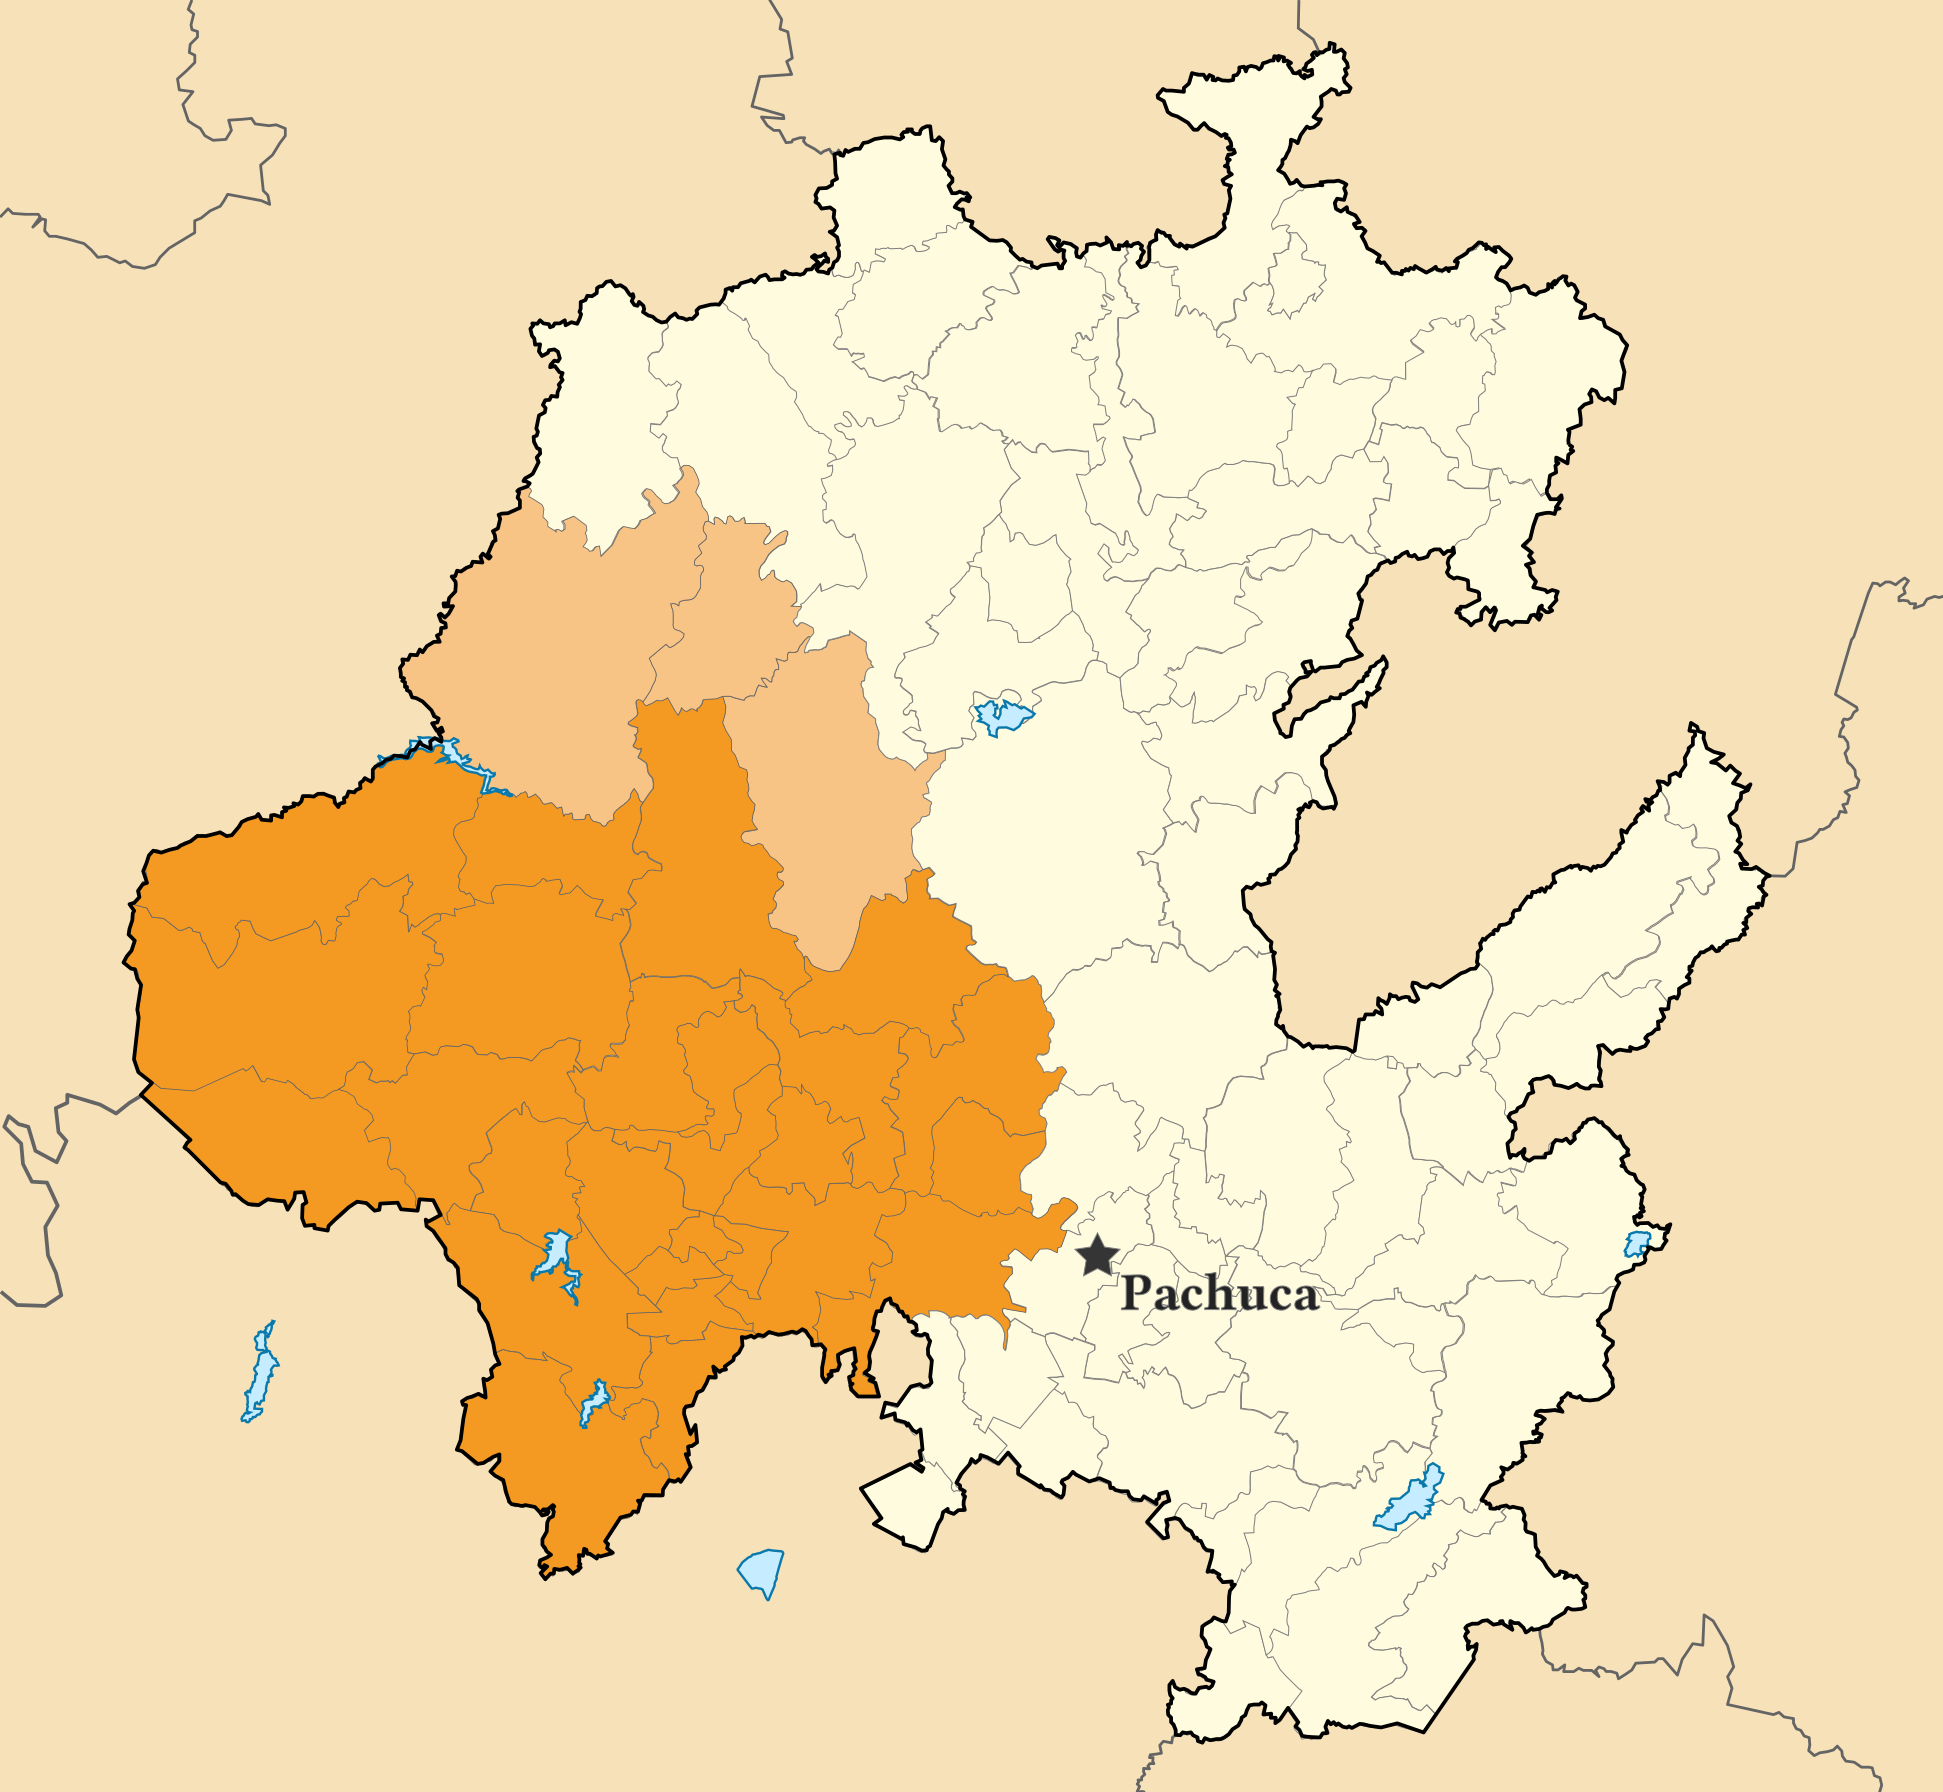
\includegraphics[width=0.8\textwidth]{../../imagenes/Mapa_Valle_del_Mezquital.svg}
    \caption{Mapa del Valle del Mezquital}
\end{figure}

\subsubsection{Hñähñus}
``La historia prehispánica del grupo Otomí es muy oscura, creyéndose durante algún tiempo que tal grupo étnico es uno de loa más antiguos de Mesoaméricica`` \cite[67]{GuerreroGuerrero1983}. Desde Cuicuilco y Copilco, hasta el Valle del Mezquital, lo Otomies o mejor conocidos por ellos mismos como Hñähñus, son una de las culturas con mas enigma en su origen y desglose desde el sur del Valle de México hasta el Valle del Mezquital pero no siendo estos los primeros habitantes del lugar.

\begin{center}
    \begin{minipage}{0.9\linewidth}
        \vspace{5pt}%margen superior de minipage
        {\small
En el Preclásico existieron pequeños asentamientos con influencia Chupícuaro y Ticoman, pero, aparentemente, la región se encontraba despoblada; durante el periodo Clásico se inició el poblamiento en el noroccidente por los grupos Xajay, con posibles herencias de Chupícuaro- Mixtlan, mientras que los grupos de filiación teotihuacana, posiblemente accediendo por el sureste del Valle, fundaron cabeceras en las inmediaciones de Tula. Para el periodo Epiclásico se abandonaron los sitios teotihuacanos y se desarrollaron sistemas autónomos vinculados con Coyotlatelco, mientras que los asentamientos Xajay permanecieron ocupados, en especial sus centros cívico-ceremoniales. En este momento se inició el poblamiento de la región árida a partir del río Tula, aunque el valle no parece haber sido densamente poblado. Con el surgimiento de la ciudad de Tula se dio un incremento poblacional en el valle que ocupó la cabecera, mientras que en el resto de la región bajó la densidad de la población, concentrándose en núcleos de asentamiento específicos. En el Posclásico Tardío la región es dominada por la Triple Alianza, se observa un fuerte incremento poblacional con la ocupación de todo el Valle mediante sistemas de asentamiento dispersos y centros ceremoniales en las cimas de los cerros. La presencia del grupo etnobiológico otomí, en estas dinámicas, es evidente desde el Epiclásico.
        }
        \begin{flushright}
            \citep[1]{aguilar2009}
        \end{flushright}
        \vspace{5pt}%margen inferior de la minipage
    \end{minipage}
\end{center}

El Valle ha sido una región en constante movimiento desde sus inicios, desde los primeros asentamientos hasta lo que lo conforma hoy en día, pero siempre manteniendo los magníficos paisajes y su vegetación, siendo esto algo por lo que las personas de muchos lugares visitan los poblados de la región.

El estudio a profundidad del origen de este grupo étnico se dificulta debido a la larga lista de grupos sociales, cambios que a sufrido la región y la perdida o falta de registros de los mismos a lo largo de la historia.

``A pesar de que el grupo otomí se asentó en la región árida del Valle del Mezquital, éste, por su ubicación y condiciones ecológicas, encerraba una variedad de hábitats y nichos. Su riqueza se hacía manifiesta en la diversidad de cactáceas, bosques de pino piñonero, agaves, yucas, mezquites, además de la nutrida fauna que frecuentaba sus chaparrales. Todo ello, combinado con el conocimiento ancestral adquirido por su contacto con los grupos nahuas, les abría la posibilidad de utilizarlo de manera variada, intensiva y acorde con los ciclos naturales.`` \citep{granados2004agricultura}

\subsubsection{Vivienda Tradicional}
La arquitectura vernácula ``no responde a estilos, no representa épocas, no necesita de arquitectos, son quienes las habitan los encargados de modelarlas, ha estado allí, testigo de la cultura de los hombres`` \citep{gonzalez2017arquitectura}. Siendo parte del patrimonio de las comunidades y asentamientos humanos desde sus inicios, inventores de este tipo de arquitectura que no surge en busca de estética, proporción o cualquier otro sentir si no por la necesidad de un refugio, hecho con los materiales que cada localidad y comunidad tenia a su alcance, haciendo lo mejor que se podía conseguir con lo que se tenia a la mano.

Sin embargo, este tipo de arquitectura a sido desplazada poco a poco debido a la marginación que la globalización junto con diferentes factores como la migración de las nuevas generaciones en las comunidades para la búsqueda de nuevas oportunidades, generan que los ideales de las personas al salir de su contexto sociocultural se mezcle con los de personas y ciudades, provocando que este quiera imitar lo que ve como nuevo y mejor en su lugar de origen, trayendo con esto un contexto muy diferente al que están acostumbrados, haciendo que las interacciones que se había entre la forma de habitar, desarrollarse y desenvolverse en su territorio, cambien radicalmente, incluso llegando a afectar sus costumbres y tradiciones, las cuales toman como algo antiguo y que pocas veces quieren mantener vivo en su forma de vida. 

Tomando en cuenta lo anterior, ``el patrimonio cultural y el patrimonio natural están cada vez más amenazados de destrucción, no sólo por las causas tradicionales de deterioro sino también por la evolución de la vida social y económica que las agrava con fenómenos de alteración o de destrucción aún más terribles''\citep{UNESCO1972}.

La transición que la vivienda ha tenido a lo largo de los años en las diferentes regiones del Valle, son diferentes de acuerdo a la localidad, comunidad, nivel económico y social de las personas, pero ``...los conocimientos tradicionales presentan el inconveniente de que, por haber sido transferidos oralmente y mediante experiencias vivénciales de una generación a otra, rara vez se cuenta con documentos que permitan su caracterización y difusión. Además, como sucede con otras costumbres populares, es común que con el paso del tiempo vayan recibiendo influencias externas o alteraciones que en ocasiones acaban por desvirtuar sus bases originales."\citep{guerrero2007arquitectura}

La arquitectura vernácula, conformada por diferentes sistemas constructivos, dependientes de la región, clima, materiales locales y contexto sociocultural es el principio de toda arquitectura, desde que el ser humano paso a ser sedentario, conformando sistemas sociales más complejos y con esto, igualmente refugios más adecuados a su forma de vida. Las construcciones eran conformadas principalmente por tierra la cual es su componente principal, mezclada con algún aglomerante de fibras vegetales, materiales que se encontraban en el lugar donde se planeaba construir. Sistemas que fueron surgiendo como parte de la experimentación con los recursos que se tenían al alcance y que pasando de generación en generación estos conocimientos, fueron mejorando cada vez más y formando tradición en cada comunidad.

Existen sistemas como el Adobe, bajareque, tapia, muros de piedra natural, paja, techos de materiales vegetales como la penca de maguey, etc. sistemas que cada comunidad adoptó y apropio, haciendo que estos fueran parte de sus conocimientos mas arraigados he importantes para cada uno, convirtiéndose en evidencia de su forma cultura y tradiciones.

``En el continente americano se ha encontrado evidencia de construcciones en tierra desde el periodo prehispánico. Con la llegada de los españoles se implementaron nuevos sistemas en los siglos XVI y XVIII empleaban sistemas como el bajareque -de tradición indígena-, la tapia y el adobe que, combinados con materiales como piedra y madera, se constituyen en la base material de la arquitectura que hoy hace parte del patrimonio cultural en nuestro continente"\citep{beltrantradicion}

\begin{figure}[ht]
    \center
    \includegraphics[width=0.8\textwidth]{../../imagenes/Organos.jpg}
    \caption{Sistema constructivo tradicional a base de órganos}
\end{figure}

Hoy en día, los sistemas industrializados en la construcción, gracias a sus ventajas en comparación con los sistemas tradicionales, como lo pueden ser, frente a los factores ambientales, el no tener que preocuparse en si mismo por la construcción ya que una persona externa se encarga de realizarla, etc. Llegando a volverse un identificador del nivel de vida de las personas en donde, en una sociedad, los sistemas tradicionales se llegan a considerar marginales o específicos de zonas rurales o lejanas a ciudades principales. Pero desde que se vieron algunos contras de los materiales industrializados como lo puede ser la contaminación y el deterioro de las zonas de donde se extraen enormes cantidades de materiales para realizarlos han resaltando los beneficios medioambientales que traen consigo los sistemas tradicionales, los cuales son sustentables, construidas con materiales naturales, con mantenimiento pueden perdurar muchos años, etc. pero como menciona \citep{gandara2000}, esta característica parece ser la única que está atrayendo al público hacia la importancia de este tipo de construcciones, incluso dejando de lado el valor cultural e histórico de su trasfondo.

La vivienda en su contexto actual se ha visto trasformada a través de cambios ideológicos y sociales provenientes de combinaciones entre grupos que migran fuera de sus lugares de origen. ``En el caso de la urbanización y la cada vez mayor tendencia a vivir en el mundo urbano influye en el deseo de las personas que no viven en las ciudades, de poseer una vivienda con referentes urbanos, aunque las formas físicas, organizativas, tecnológicos y usos no se correspondan con sus costumbres culturales."\citep{alvarez2003maguey},

\section{ChatGPT}
La civilización otomí es una cultura mesoamericana que se desarrolló en la región central de México desde la época prehispánica hasta la llegada de los españoles en el siglo XVI. Los otomíes eran un pueblo agrícola que se dedicaba principalmente a la cultivo de maize, frijoles y chiles, y vivían en aldeas y pequeñas ciudades gobernadas por jefes locales.

Durante el período prehispánico, los otomíes mantuvieron relaciones comerciales y políticas con otras culturas mesoamericanas, como los mexicas y los tecuexes, y formaron parte de la Gran Alianza Mexicana, una confederación de pueblos indígenas que se unieron para resistir la invasión de los tecuexes.

Con la llegada de los españoles en el siglo XVI, la vida de los otomíes cambió drásticamente. Fueron sometidos por los conquistadores y obligados a trabajar en las encomiendas, donde eran explotados y maltratados. Además, la introducción de enfermedades europeas y la imposición de la religión católica disminuyó la población otomí significativamente.

Sin embargo, los otomíes no perdieron completamente su cultura y tradiciones. Muchos de sus mitos, creencias y costumbres sobrevivieron hasta el día de hoy y continúan siendo transmitidos de generación en generación.

Hoy en día, los descendientes de los otomíes en México mantienen una fuerte identidad cultural y participan activamente en la preservación de su patrimonio y tradiciones. Su arte, música y danzas continúan siendo una parte importante de la cultura mexicana y son reconocidos a nivel nacional e internacional.
